\chapter{Visualization and Debugging}\indexmain{Debugger}
\label{chapdebugger}

This chapter gives an introduction into the visualization capabilites of yComp and into the graphical debugger of \GrG, which is offered by \GrShell\ in combination with yComp.

Other commands of use for debugging were already introduced in the shell chapter:
\verb#show var <Variable># to print the content of a variable (but pressing the \texttt{v} key in the shell debugger is a lot more convenient) and \verb#show <GraphElement>.<AttributeName># to print the content of an attribute (but searching with \texttt{Ctrl-f} or \texttt{/} in yComp for the persistent name or an attribute value, hovering over the then highlighted graph element is more convenient, again); furthermore \verb#record# and \verb#replay# are interesting when you are debugging a transformation where you are choosing from the available matches by hand and want to try other paths later by choosing differently on a previous match: they allow you to save and restore graph states of interest, and to inspect the sequence of changes which lead to them in the \texttt{.grs}.

%%%%%%%%%%%%%%%%%%%%%%%%%%%%%%%%%%%%%%%%%%%%%%%%%%%%%%%%%%%%%%%%%%%%%%%%%%%%%%%%%%%%%%%%%%%%%%%%
\section{Graph Visualization Commands (Nested Layout)}\label{sub:visual}\indexmain{visualization}\indexmainsee{layout}{visualization}\indexmainsee{visualization}{group node}\indexmain{nested layout}\indexmainsee{nested layout}{group node}\indexmain{nested graph}\indexmainsee{nested graph}{group node}

\begin{rail}
  'show' 'graph' ExecutableName (() | Text)
\end{rail}\ixkeyw{show}\ixkeyw{graph}
Dumps the current graph in \indexed{VCG} format into a temporary file.
The temporary VCG file will be passed to the program \emph{ExecutableName} as first parameter;
further parameters, such as program options, can be specified by \emph{Text}.
If you use \yComp\footnote{See Section~\ref{tools:ycomp}.}\indexmain{yComp} as executable (\texttt{show graph ycomp}), this may look like
\begin{center}
  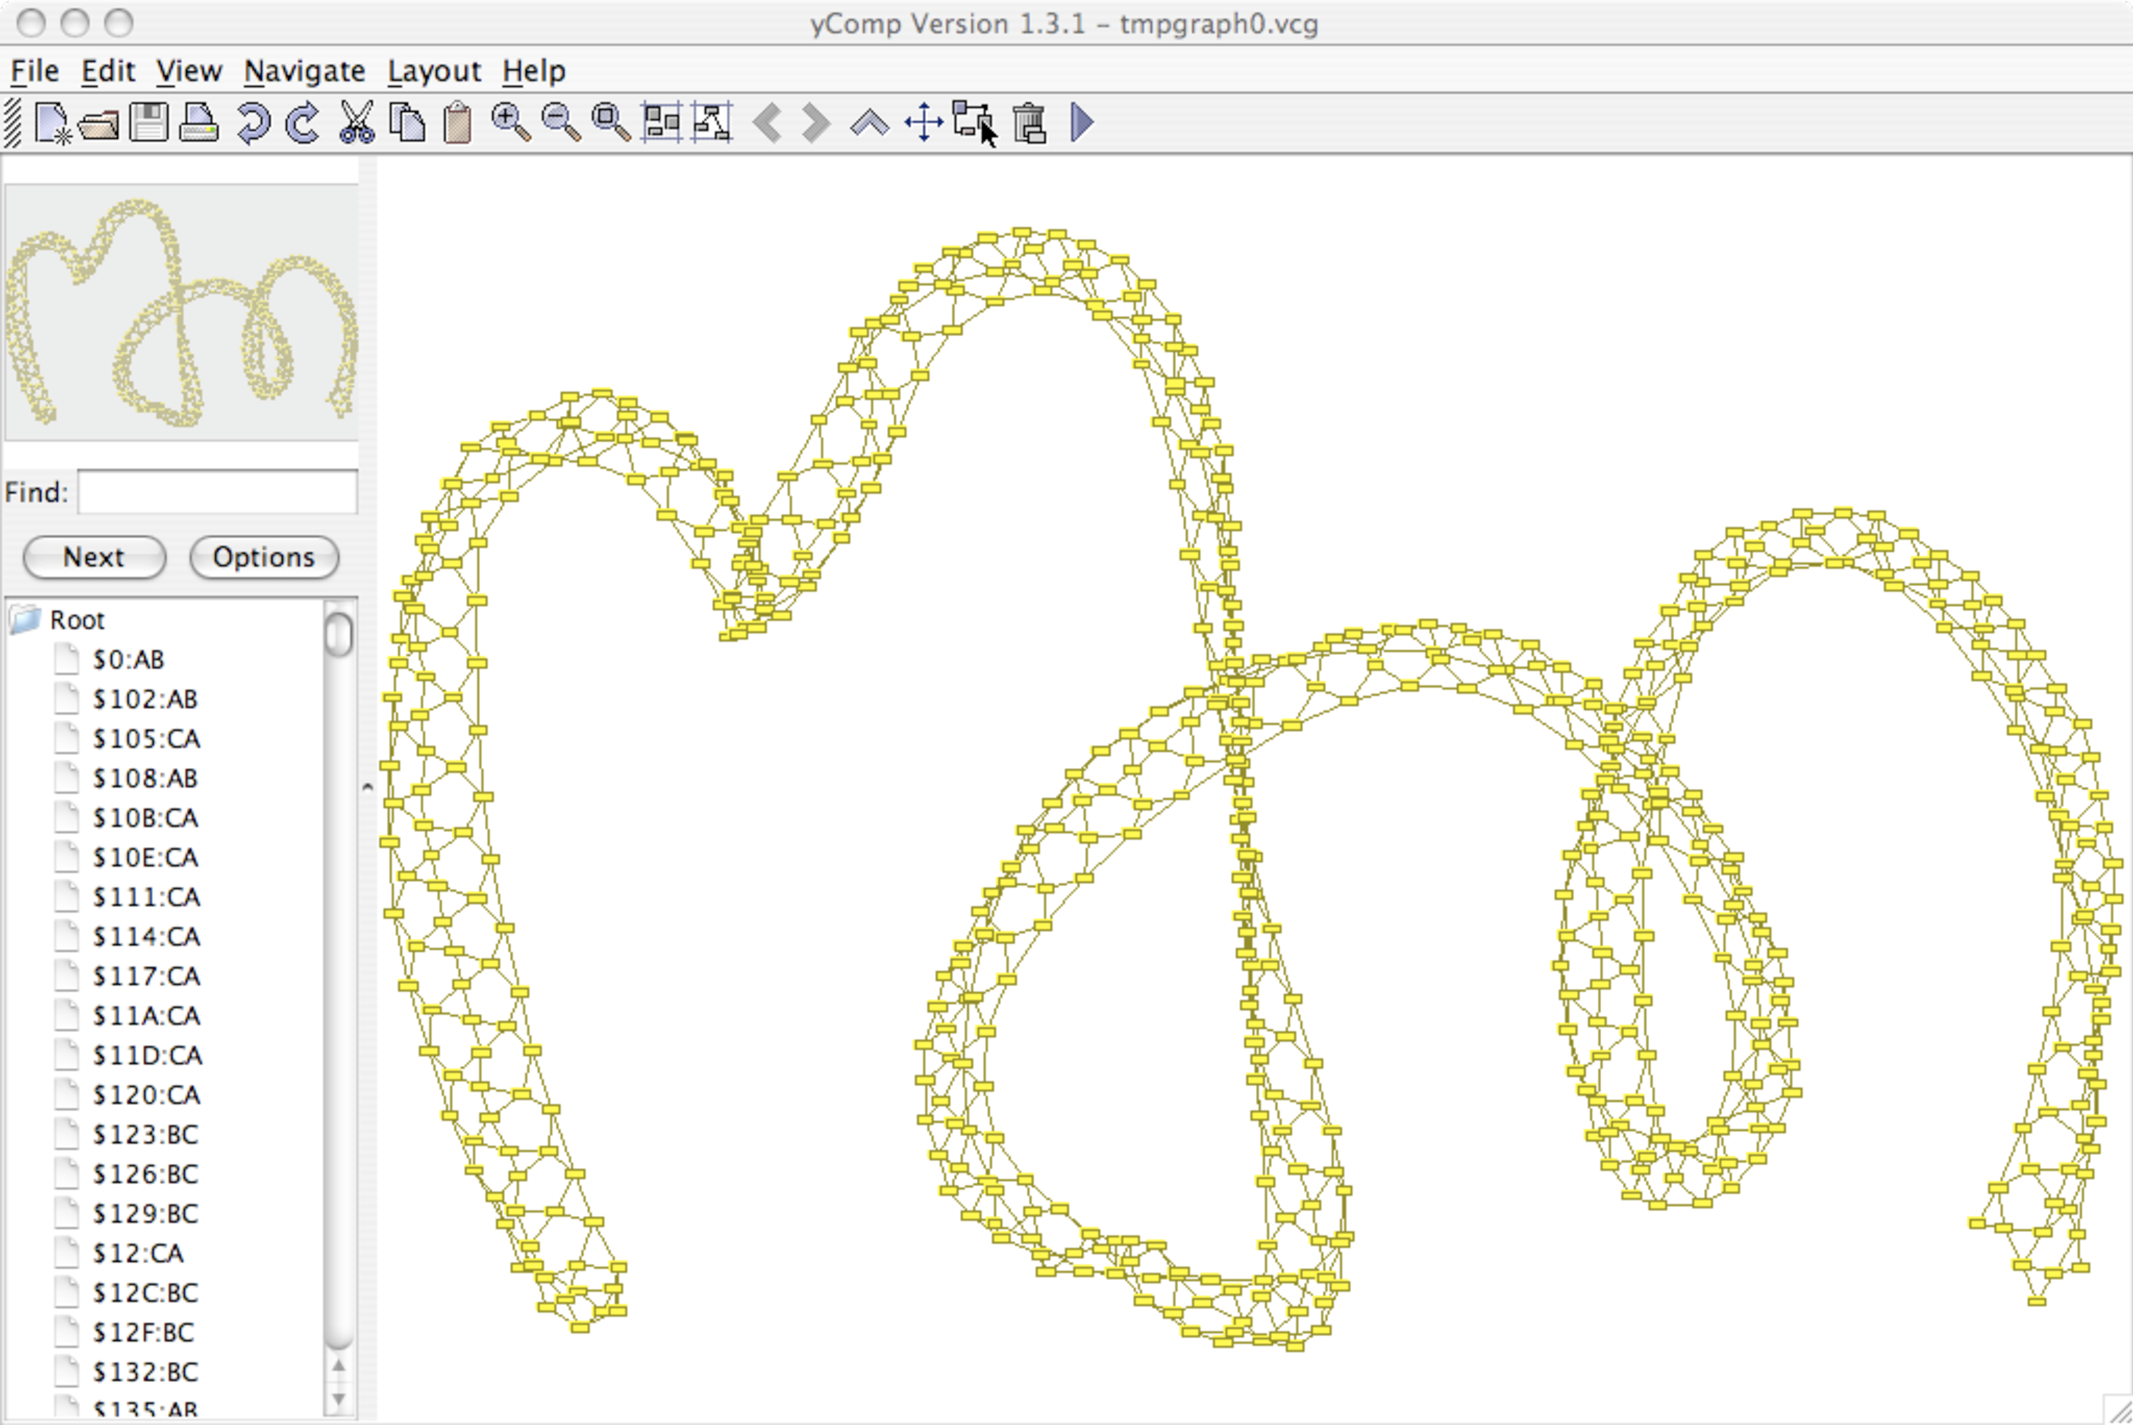
\includegraphics[width=0.75\linewidth]{fig/showgraph}
\end{center}
The temporary file will be deleted, when the application \emph{Filename} is terminated if \GrShell\ is still running at this time.

\begin{rail}
  'dump' 'graph' Filename
\end{rail}\ixkeyw{dump}\ixkeyw{graph}
Dumps the current graph in \indexed{VCG} format into the file \emph{Filename}.\\

The following commands control the style of the VCG output. This affects \texttt{dump graph}, \texttt{show graph}, and \texttt{enable debug}.
\begin{rail}
  'dump' 'set' 'node' (() | 'only') NodeType DumpNodeContinuation;
DumpNodeContinuation:
 (('color' | 'textcolor' | 'bordercolor') Color | 'shape' Text | 'labels' ('on' | 'off' | Text)) ;
\end{rail}\ixkeyw{dump}\ixkeyw{set}\ixkeyw{node}\ixkeyw{only}\ixkeyw{color}\ixkeyw{textcolor}\ixkeyw{bordercolor}\ixkeyw{shape}\ixkeyw{labels}\ixkeyw{on}\ixkeyw{off}\ixnterm{DumpNodeContinuation}
Sets the \indexed{color}, text color, border color, the shape or the label of the nodes of type \emph{NodeType} and all of its subtypes.
The keyword \texttt{only} excludes the subtypes. The available colors are specified at the begin of this chapter.
The following shapes are supported: \texttt{box}, \texttt{triangle}, \texttt{circle}, \texttt{ellipse}, \texttt{rhomb}, \texttt{hexagon}, \texttt{trapeze}, \texttt{uptrapeze}, \texttt{lparallelogram}, \texttt{rparallelogram}.
Those are shape names of \yComp\ (for a VCG definition see~\cite{vcg}).
The following colors are supported: \texttt{Black}, \texttt{Blue}, \texttt{Green}, \texttt{Cyan}, \texttt{Red}, \texttt{Purple}, \texttt{Brown}, \texttt{Grey}, \texttt{LightGrey}, \texttt{LightBlue}, \texttt{LightGreen}, \texttt{LightCyan}, \texttt{LightRed}, \texttt{LightPurple}, \texttt{Yel\-low} (default), \texttt{White}, \texttt{DarkBlue}, \texttt{DarkRed}, \texttt{Dark\-Green}, \texttt{DarkYellow}, \texttt{DarkMagenta}, \texttt{DarkCyan}, \texttt{Gold}, \texttt{Lilac}, \texttt{Turquoise}, \texttt{Aquamarine}, \texttt{Khaki}, \texttt{Pink}, \texttt{Orange}, \texttt{Orchid}, \texttt{LightYellow}, \texttt{YellowGreen}.
These are the same color identifiers as in \indexed{VCG}/\yComp\ files (for a VCG definition see~\cite{vcg}).

The default labeling is set to \texttt{on} with \texttt{Name:Type}, it can be overwritten by an specified label string (e.g. the source code line originating the node in a program graph) or switched off.

\begin{rail}
  'dump' 'set' 'edge' (() | 'only') EdgeType DumpEdgeContinuation;
DumpEdgeContinuation:
  (('color' | 'textcolor') Color | 'linestyle' (Text) | 'thickness' (Number) | 'labels' ('on' | 'off' | Text));
\end{rail}\ixkeyw{dump}\ixkeyw{set}\ixkeyw{edge}\ixkeyw{only}\ixkeyw{color}\ixkeyw{textcolor}\ixkeyw{labels}\ixkeyw{on}\ixkeyw{off}\ixkeyw{linestyle}\ixkeyw{thickness}\ixnterm{DumpEdgeContinuation}
Sets the color, text color, the linestyle, the thickness of the line, or the label of the edges of type \emph{EdgeType} and all of its subtypes.
The keyword \texttt{only} excludes the subtypes. The available colors are specified above.
The default labeling is set to \texttt{on} with \texttt{Name:Type}, it can be overwritten by an specified label string or switched off.
The following linestyles are supported: \texttt{continuous} (default), \texttt{dotted}, \texttt{dashed}.
The following thicknesses are supported: \texttt{1} (default), \texttt{2}, \texttt{3}, \texttt{4}, \texttt{5}.

\begin{rail}
  'dump' 'add' (('node' ('only')? NodeType)|('edge' ('only')? EdgeType)) 'exclude' ;
\end{rail}\ixkeyw{dump}\ixkeyw{add}\ixkeyw{node}\ixkeyw{edge}\ixkeyw{only}\ixkeyw{exclude}
Excludes nodes/edges of type \emph{NodeType}/\emph{EdgeType} and all of its subtypes from output, for a node it also excludes its incident edges.
The keyword \texttt{only} excludes the subtypes from exlusion, i.e.\ subtypes of \emph{NodeType}/\emph{EdgeType} are dumped.

\begin{rail}
  'dump' 'add' 'node' ('only')? NodeType 'group' (GroupConstraints)? ;
GroupConstraints:
  'by' ('hidden')? GroupMode (IncAdjTypeConstraints)? ;
IncAdjTypeConstraints:
  ('only')? EdgeType ('with' ('only')? NodeType)? ;
\end{rail}\ixkeyw{dump}\ixkeyw{add}\ixkeyw{node}\ixkeyw{only}\ixkeyw{group}\ixkeyw{by}\ixkeyw{hidden}\ixkeyw{with}\ixnterm{GroupConstraints}\ixnterm{IncAdjTypeConstraints}
Declares \emph{NodeType} and subtypes of \emph{NodeType} as \indexed{group node}\indexmainsee{hierarchic}{group node} type.
All the differently typed nodes that point to a node of type \emph{NodeType}
(i.e.\ there is a directed edge between such nodes) will be grouped and visibly enclosed by the \emph{NodeType}-node (nested graph).
\texttt{GroupMode} is one of \texttt{no},\texttt{incoming},\texttt{outgoing},\texttt{any}; \texttt{hidden} causes hiding of the edges by which grouping happens.
The \texttt{EdgeType} constrains the type of the edges which cause grouping, the \texttt{with} clause additionally constrains the type of the adjacent node;
\texttt{only} excludes subtypes.

\begin{warning}
Only apply group commands on a graph if they indeed lead to a containment tree of groups.
If the group commands would lead to a directed acyclic or even cyclic containment graph, the results are undefined.
You may get duplicate edges (and nodes); the implementation is free to choose indeterministically between the possible nestings -- it may even grow an arm and stab you in your back.
(A conflict resultion heuristic used is to give the earlier executed \texttt{add group} command priority.
But this mechanism is incomplete -- you'd better refine your groups or change the model in that case.
Using a model separating edges denoting direct containment from cross-linking edges by type is normally the better design, even disregarding visual node nesting.)
\end{warning}

The following example shows \emph{metropolis} ungrouped and grouped:
\begin{center}
  \fbox{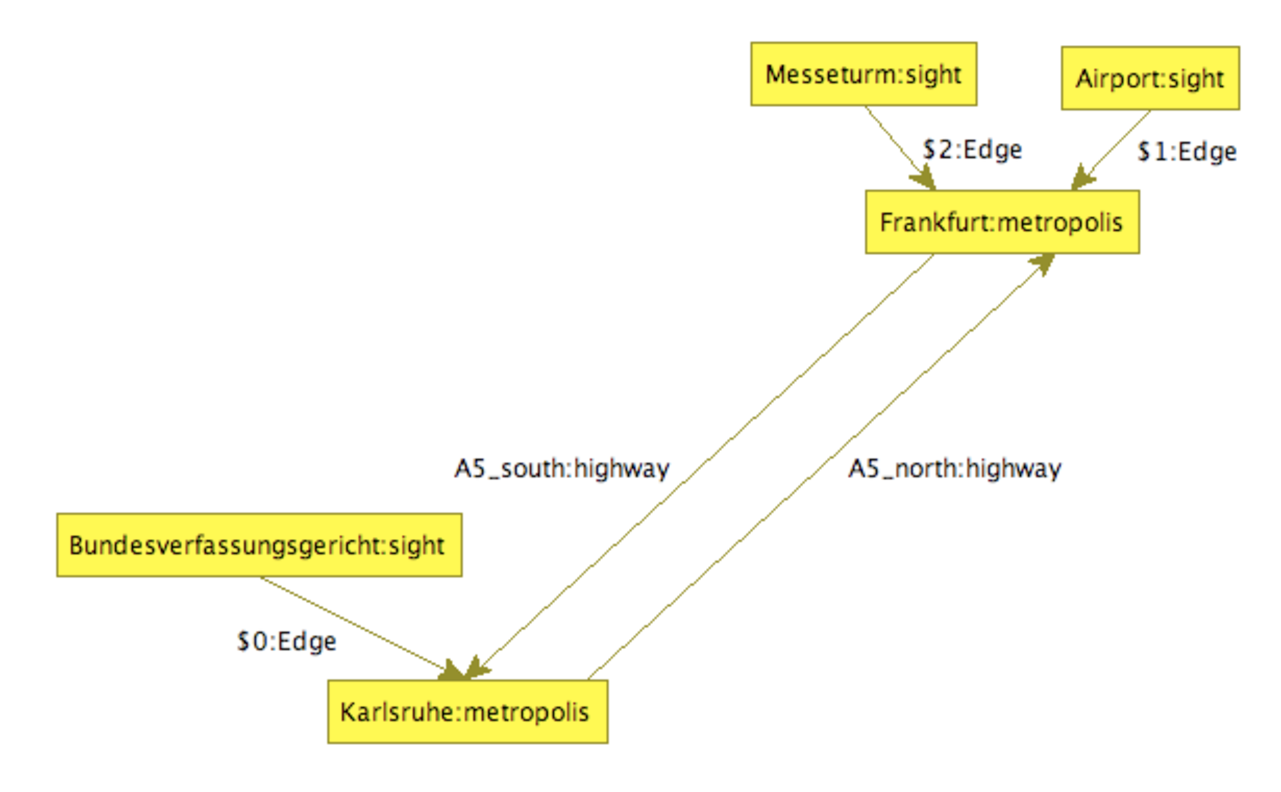
\includegraphics[width=0.45\linewidth]{fig/group2-1}}  \hfill \fbox{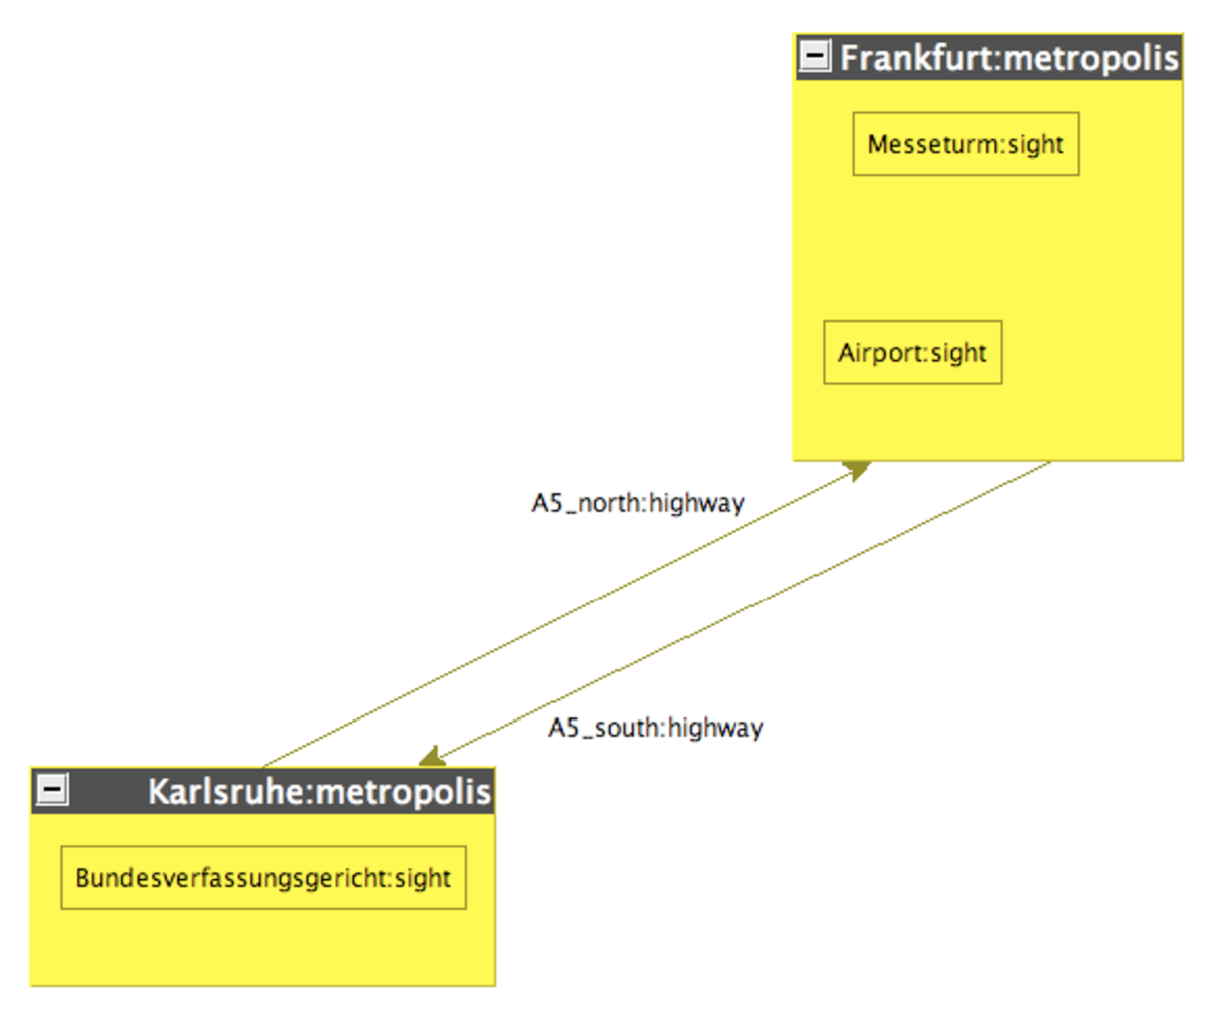
\includegraphics[width=0.45\linewidth]{fig/group2-2}}\\
  {\small right side: dumped with \texttt{dump add node metropolis group}}
\end{center}

\begin{rail}
  'dump' 'add' (() | 'only') ('node' NodeType | 'edge' EdgeType) \\ ('infotag' | 'shortinfotag') AttributeName
\end{rail}\ixkeyw{dump}\ixkeyw{add}\ixkeyw{only}\ixkeyw{node}\ixkeyw{edge}\ixkeyw{infotag}\ixkeyw{shortinfotag}
Declares the \indexed{attribute} \emph{AttributeName} to be an ``\indexed{info tag}'' or ``\indexed{short info tag}''.
Info tags are displayed like additional node/edge \indexed{label}s, in format \texttt{Name=Value}, or \texttt{Value} only for short info tags.
The keyword \texttt{only} excludes the subtypes of \emph{NodeType} resp.\ \emph{EdgeType}.
In the following example \emph{river} and \emph{jam} are info tags:
\begin{center}
  \fbox{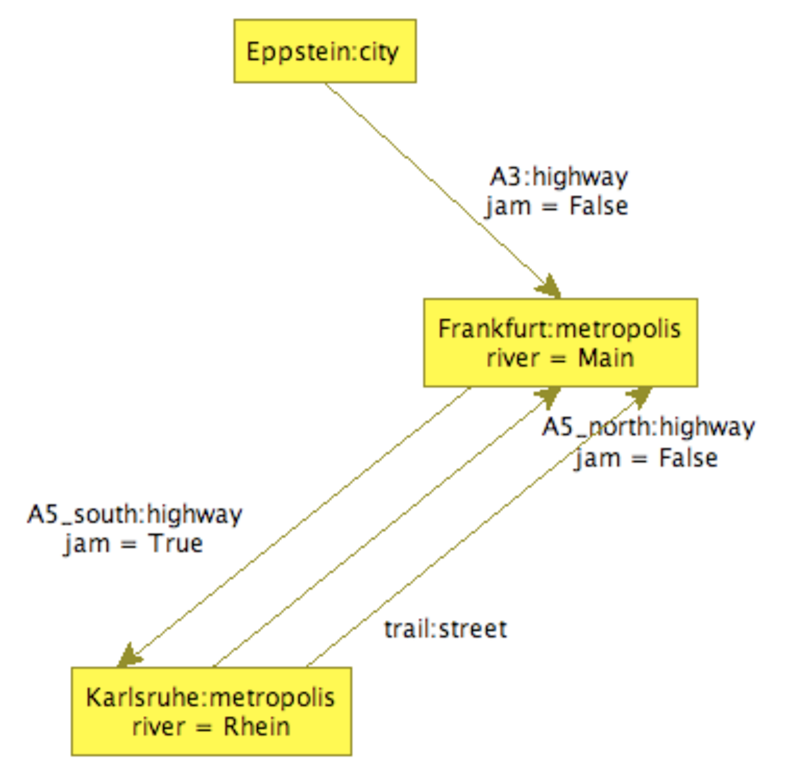
\includegraphics[width=0.5\linewidth]{fig/infotag}}
\end{center}

\begin{rail}
  'dump' 'reset'
\end{rail}\ixkeyw{dump}\ixkeyw{reset}
Resets all style options (\texttt{dump set}\dots) and (\texttt{dump add}\dots) to their default values.


\begin{note}\label{note:visual}
Small graphs allow for fast visual understanding, but with an increasing number of nodes and edges they quickly loose this property.
The group commands are of outstanding importance to keep readability with increasing graph sizes
(e.g. for program graphs it allows to lump together expressions of a method inside the method node and attributes of the class inside the class node).
Additional helpers in keeping the graph readable are:
the capability to exclude elements from dumping (the less hay in the stack the easier to find the needle),
the different colors and shapes to quickly find the elements of interest,
as well as the labels/infotags/shortinfotags to display the most important information directly.
Choose the layout algorithm and the options delivering the best results for your needs, organic and hierarchic or compiler graph
(an extension of hierarchic with automatic edge cutting -- marking cut edges by fat dots, showing the edge only on mouse over and allowing to jump to the other end on a mouse click)
should be tried first.
\end{note}

The following example shows several of the layout options employed to considerably increase the readability of a program graph (as given in \texttt{examples/JavaProgramGraphs-GraBaTs08}):
\begin{figure}[htbp]
  \centering
  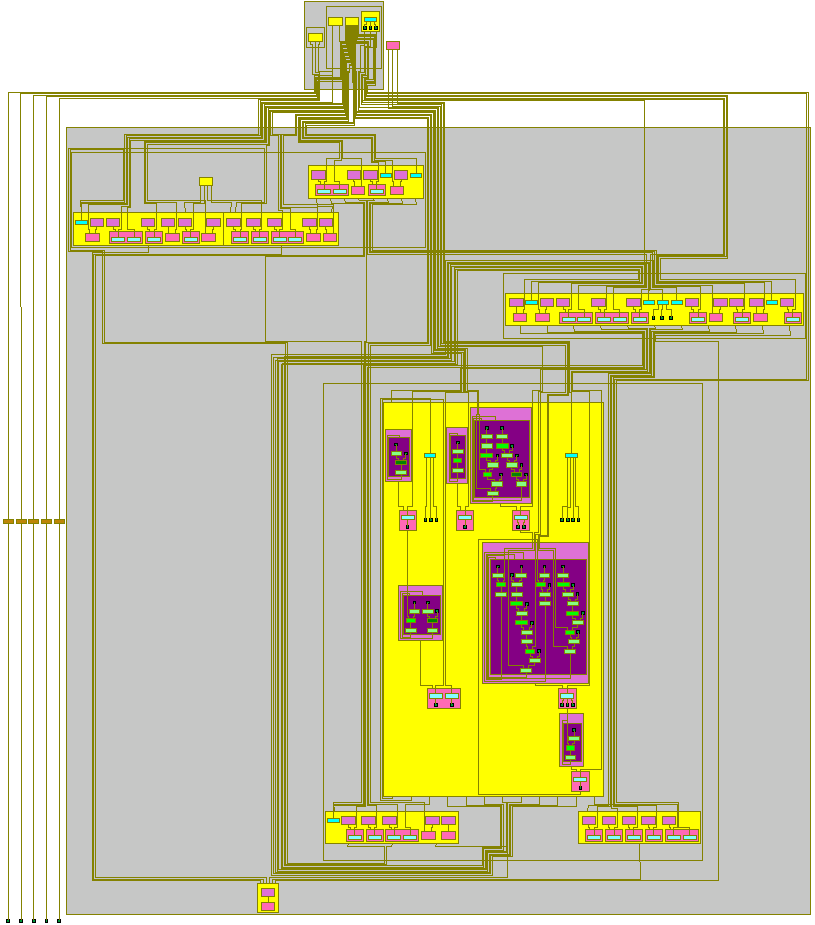
\includegraphics[width=0.99\textwidth]{fig/screen-overview}
  \caption{Overview of the initial program graph }
  \label{figprogramgraph1}
\end{figure}

\begin{figure}[htbp]
  \centering
  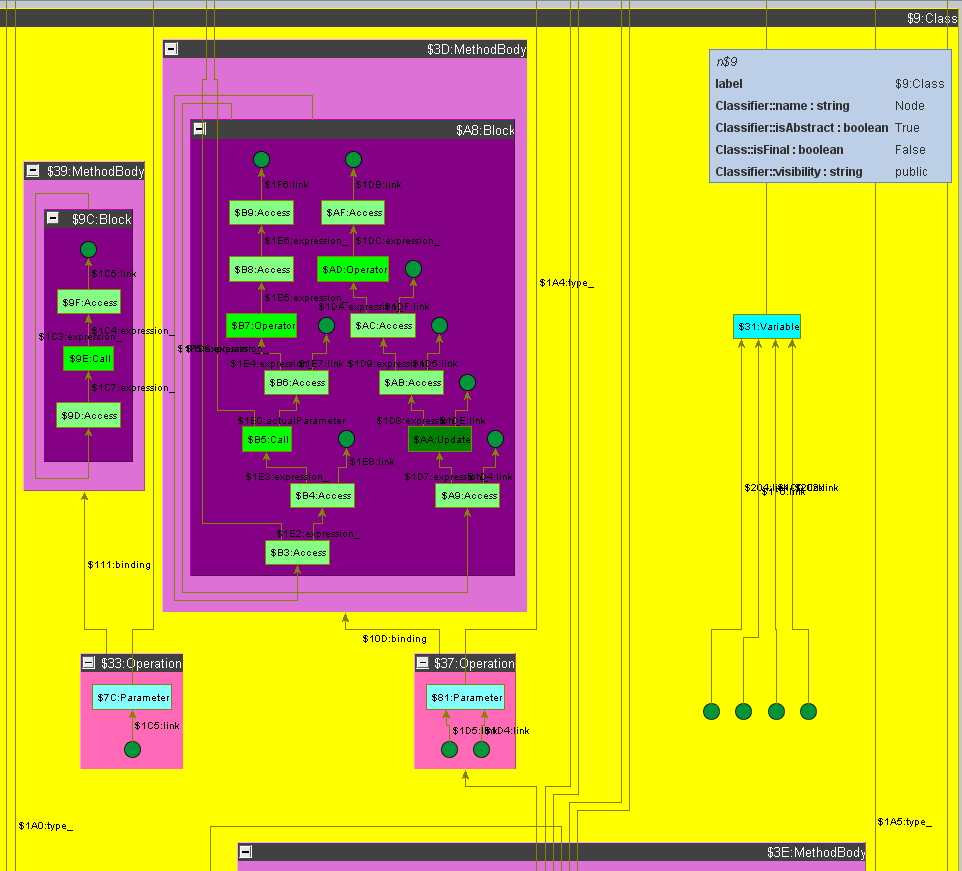
\includegraphics[width=0.99\textwidth]{fig/screen-detail}
  \caption{Some details of the ``Node'' class of the initial program graph}
  \label{figprogramgraph2}
\end{figure}

\pagebreak 

%%%%%%%%%%%%%%%%%%%%%%%%%%%%%%%%%%%%%%%%%%%%%%%%%%%%%%%%%%%%%%%%%%%%%%%%%%%%%%%%%%%%%%%%%%%%%%%%
\section{Debugging Related Commands}

\begin{rail}
  'debug' ( 'enable' | 'disable' )
\end{rail}\ixkeyw{debug}\ixkeyw{enable}\ixkeyw{disable}
Enables and disables the \indexed{debug mode}.
The debug mode shows the current working graph in a \yComp\ window.
All changes to the working graph are tracked by \yComp\ immediately.

\begin{rail}
  'debug' 'set' 'layout' ( (Text)? | 'option' Name String ) ;
\end{rail}\ixkeyw{debug}\ixkeyw{set}\ixkeyw{layout}\ixkeyw{option}
Sets the default graph \indexed{layout algorithm} to \emph{Text}.
If \emph{Text} is omitted, a list of the available layout algorithms is displayed.
The following layout algorithms are supported: \texttt{Random}, \texttt{Hierarchic}, \texttt{Organic}, \texttt{Orthogonal}, \texttt{Circular}, \texttt{Tree}, \texttt{Diagonal}, \texttt{Incremental Hierarchic}, \texttt{Compilergraph}.
For technical graphs \texttt{Hierarchic} works normally best; \texttt{Compilergraph} is a version of \texttt{Hierarchic} cutting some edges, it may be of interest if \texttt{Hierarchic} contains too many crossing edges. \texttt{Organic} is the other general purpose layout available, the other layouts are rather special, but this should not prevent you from using them if they fit to your task ;).
The \texttt{option} version allows to specify layout options by name value pairs.
The available layout options can be listed by the following command.

\begin{rail}
  'debug' 'get' 'layout' 'options';
\end{rail}\ixkeyw{debug}\ixkeyw{get}\ixkeyw{layout}\ixkeyw{options}
Prints a list of the available layout options of the layout algorithm.

\begin{rail}
  'debug' 'layout';
\end{rail}\ixkeyw{debug}\ixkeyw{layout}
Forces re-layout of the graph shown in yComp (same as pressing the play button within yComp).

\begin{rail}
  'debug' 'set' 'node' 'mode' Text DumpNodeContinuation ;
\end{rail}\ixkeyw{debug}\ixkeyw{set}\ixkeyw{mode}
\begin{rail}
  'debug' 'set' 'edge' 'mode' Text DumpEdgeContinuation ;
\end{rail}\ixkeyw{debug}\ixkeyw{set}\ixkeyw{mode}
Configures the display of the visual debug states for the nodes/edges.
The following modes are supported: \texttt{matched}, \texttt{created}, \texttt{deleted}, \texttt{retyped}.
Change this if you e.g. want the matched elements to be marked more visibly, or added/deleted elements to be colored green/red.

\begin{rail}
  GraphRewriteSequence: 'debug' ('exec'|'xgrs') SimpleRewriteSequence ;
\end{rail}\ixkeyw{debug}\ixkeyw{exec}\ixkeyw{xgrs}\indexmain{graph rewrite sequence}\indexmainsee{GRS}{graph rewrite sequence}\ixnterm{GraphRewriteSequence}
This executes the graph rewrite sequence \emph{SimpleRewriteSequence} in the debugger\indexmain{debugger}.
Same as \texttt{exec SimpleRewriteSequence} in the previous chapter, but allows tracing the rewriting process step-by-step.


%%%%%%%%%%%%%%%%%%%%%%%%%%%%%%%%%%%%%%%%%%%%%%%%%%%%%%%%%%%%%%%%%%%%%%%%%%%%%%%%%%%%%%%%%%%%%%%%
\section{Using the Debugger}

The debugging process follows of a series of debug situations,
which result from a user selection of the underlying execution situations accoring to interest.
During each debugging step the debugger\indexmain{debugger} -- which is a part of the \GrShell~--
prints the debugged sequence with the currently focused/active rule highlighted yellow.
What will be shown from executing this rule depends on the commands chosen by the user;
and on the fact whether the focused rule matches or not.
An active rule which is already known to match is highlighted green.
The rules which matched during sequence execution are shown on dark green background,
the rules which failed during sequence execution are shown on dark red background;
at the begin of a new loop iteration the highlighting state of the contained rules is reset.
During execution \yComp\footnote{Make sure, that the path to your \texttt{\indexed{yComp.jar}} package is set correctly in the \texttt{ycomp} shell script within \GrG's \texttt{/bin} directory.}\indexmain{yComp}
will display the changes to the graph from every single step.
Besides deciding on what is shown from the execution of the current rule,
the user determines with the debug commands where to continue the execution
(the rule focused next; but again this depends on success/failure of the currently active rule).
The debug commands are given in Table~\ref{tabdebug}.
A run is shown in the following example \ref{ex:debug}.

In addition to the commands for actively stepping or skipping through the sequence exection,
there are breakpoints and choicepoints available (toggled with the \texttt{b} and \texttt{c} commands)
which are only processed when they are reached, but on the other hand are also processed if a user command would skip them.
The \indexed{break point}s halt execution, focus the reached sequence, and cause the debugger to wait for further commands
(e.g. \texttt{d} to inspect the rule execution en detail versus \texttt{s} for just applying it).
The \indexed{choice point}s halt execution, focus the reached sequence in magenta, and ask for some user input;
after the input was received, execution continues according to the command previously issued.
Both break points and choice points are denoted by the \texttt{\%} modifier.
The \texttt{\%} modifier works as a break point if it is given before: a rule, an all bracketed rule, a variable predicate, or the constants \texttt{true}/\texttt{false}.
The \texttt{\%} modifier works as a choice point if it is appended to the \texttt{\$} randomize modifier switching a random decision into a user decision.
This holds for the binary operators, the random match selector of all bracketed rules, the random-all-of operators and the one-of-set braces.
The idea behind this is: you need some randomization for \indexed{simulation} purposes --- then use the randomize modifier \texttt{\$}.
You want to force a certain decision overriding the random decision to try out another execution path while debugging the simulation flow --- then modify the randomize modifier with the user (choice) modifier \texttt{\%}.

The initial breakpoint and choicepoint assignment is given with the \texttt{\%} characters in the sequences after the \texttt{debug exec} commands in the \texttt{.grs} file.
The breakpoint and choicepoint commands of the debugger allow to toggle them at runtime, overriding the initial assignment (notationally yielding a sequence with added or removed \texttt{\%} characters).
The user input commands \texttt{\$\%(type)} define choice points which can't be toggled off.

Further commands allow to print the variables at a given situation, the sequence call stack, or a full state dump of the call stack and the variables.
Or allow to highlight elements in the graph, defined by being contained in a (possibly container valued) variable, or being visited according to a visited flag.

\pagebreak

\begin{table}[htbp]
  \begin{tabularx}{\linewidth}{|lX|}
\hline
  \texttt{s}(tep) & Execute the current rewrite rule (match, and rewrite in case it matched; the resulting graph is shown).\\
  \texttt{d}(etailed step) & Execute the current rewrite rule in a three-step procedure: matching - highlighting the found match, rewriting - highlighting the changing elements, and application - doing the rewrite showing the resulting graph. In addition, afterwards the execution of subrules from embedded sequences (\texttt{exec}) is shown step by step. \\
  (step) \texttt{o}(ut) & Continue execution until the end of the current loop. If the execution is not in a loop at this moment, but in a sequence called, the called sequence will be executed until its end. If neither is the case, the complete sequence will be executed.\\
  (step) \texttt{u}(p) & Ascend one level up within the \indexed{Kantorowitsch tree} of the current rewrite sequence (i.e. rule; see Example~\ref{ex:debug}; at the moment the command is pretty useless because only the serialized form is displayed).\\
  \texttt{r}(un) & Continue execution (until the end or a breakpoint).\\
  \texttt{a}(bort) & Cancel the execution immediately.\\
  \texttt{n}(ext) & Go to the next rewrite rule which matches, make it current.\\
\hline
  (toggle) \texttt{b}(reakpoint) & Toggle a breakpoint at one of the breakpointable locations.\\
  (toggle) \texttt{c}(choicepoint) & Toggle a choicepoint at one of the choicepointable locations.\\
\hline
  \texttt{v}(ariables) & Prints the global variables and the local variables of the sequence currently executed, which is the topmost sequence of the sequence call stack. Plus the allocated visited flags. To be more precise regarding local variables: all variables which were defined (and have not fallen out of scope again) up to the sequence position focussed.\\
  \texttt{t}(race) & Prints the stack trace of the current sequence call stack; the stack trace includes the body of each sequence called at its execution state.\\
  \texttt{f}(ull dump) & Prints the stack trace including the local variables of each stack frame plus the global variables.\\
  \texttt{h}(ighlight)\label{highlight} & Highlights the elements in the graph which are marked with the visited flag given, or are contained in the variable given (which might be a simple scalar variable containing a graph element, or a set/map/array valued container of graph elements). Multiple variables of visited flags may be given separated by commas.\\
\hline
  \end{tabularx}
  \caption{\GrShell\ debug commands}
  \label{tabdebug}
\end{table}
%\begin{figure}[htbp]
%  \centering
%  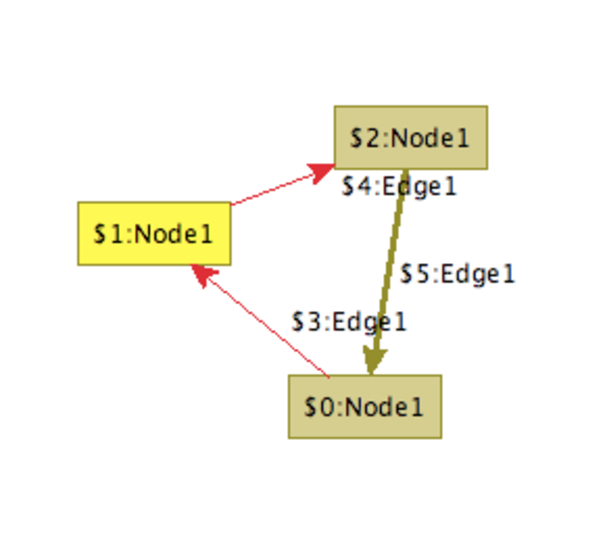
\includegraphics[width=0.25\linewidth]{fig/debug1}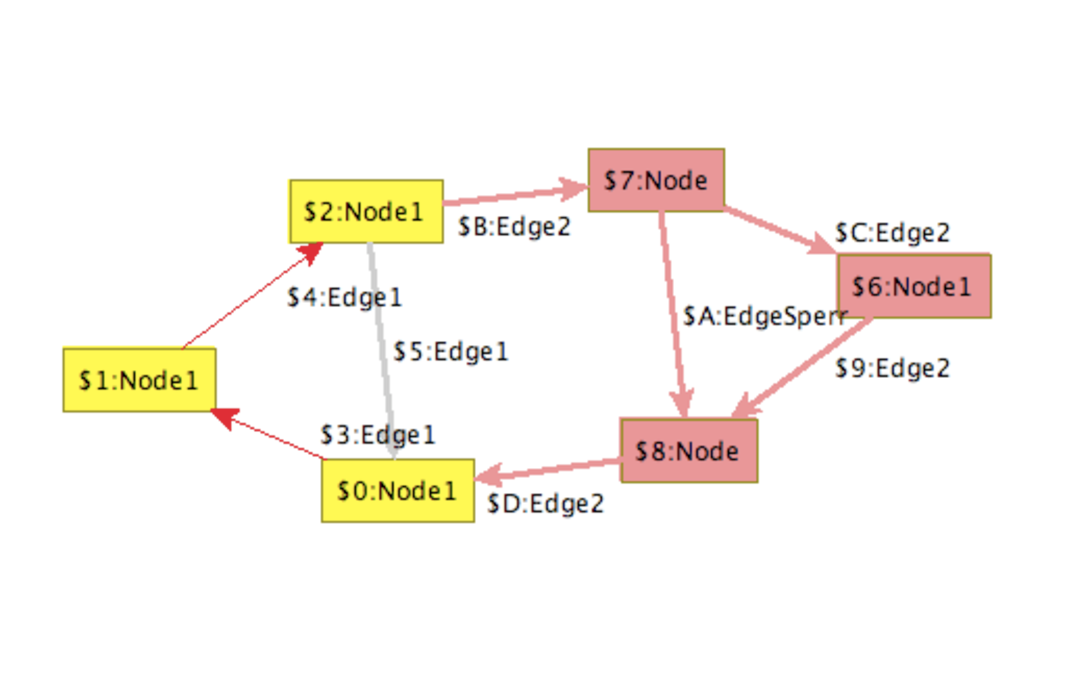
\includegraphics[width=0.4\linewidth]{fig/debug2}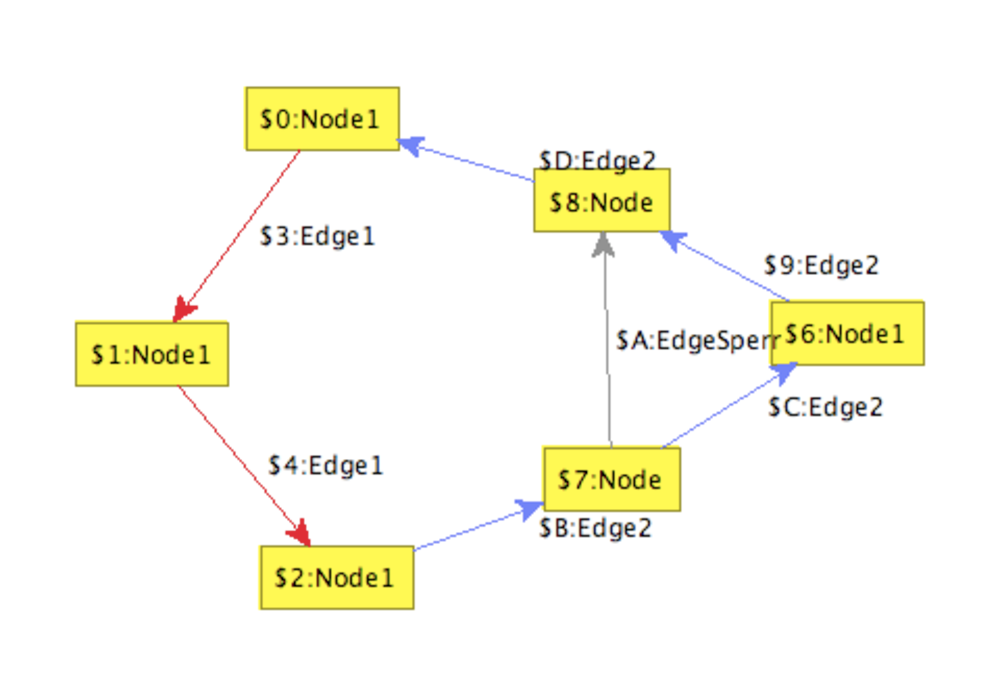
\includegraphics[width=0.4\linewidth]{fig/debug3}
%  \caption{Delayed step rule application.}
%  \label{figdebug}
%\end{figure}

\pagebreak

\begin{figure}[htbp]
\begin{example}\label{ex:debug}
We demonstrate the debug commands with a slightly adjusted script for the Koch snowflake from \GrG's examples (see also Section~\ref{fractals}). The graph rewriting sequence is
\begin{grshell}
debug exec (makeFlake1* & (beautify & doNothing)* & makeFlake2* & beautify*)[1]
\end{grshell}
\yComp\ will be opened with an initial graph (resulting from \texttt{grs init}):
\begin{center}
  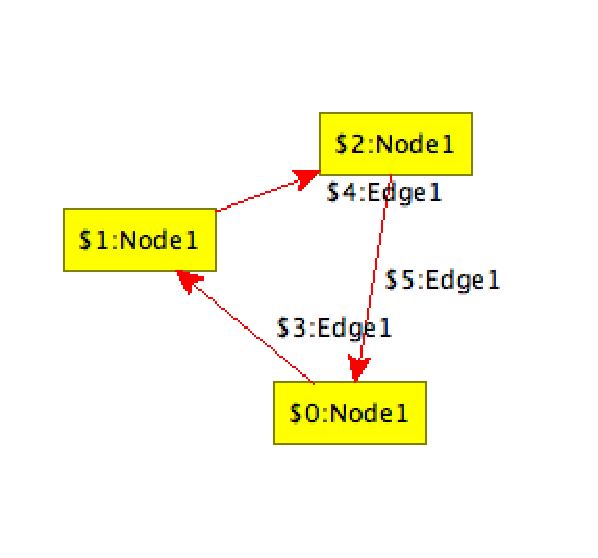
\includegraphics[width=0.3\linewidth]{fig/debug0tra}
\end{center}
We type \texttt{d}(etailed step) to apply \texttt{makeFlake1} step by step resulting in the following graphs:
\begin{center}
  \parbox{0.2\linewidth}{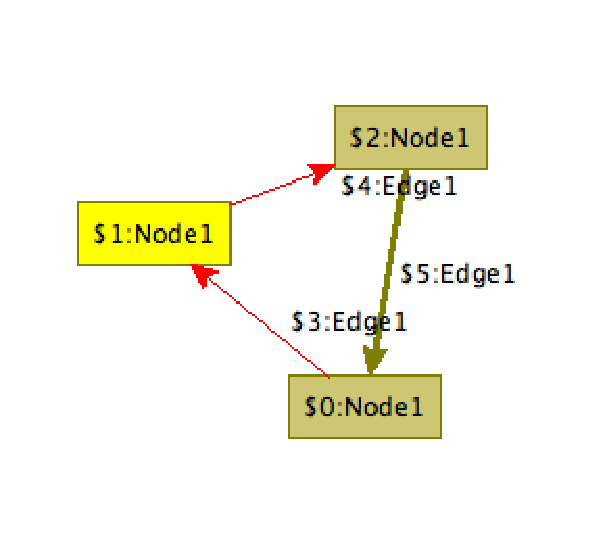
\includegraphics[width=\linewidth]{fig/debug1tra}}\parbox{0.375\linewidth}{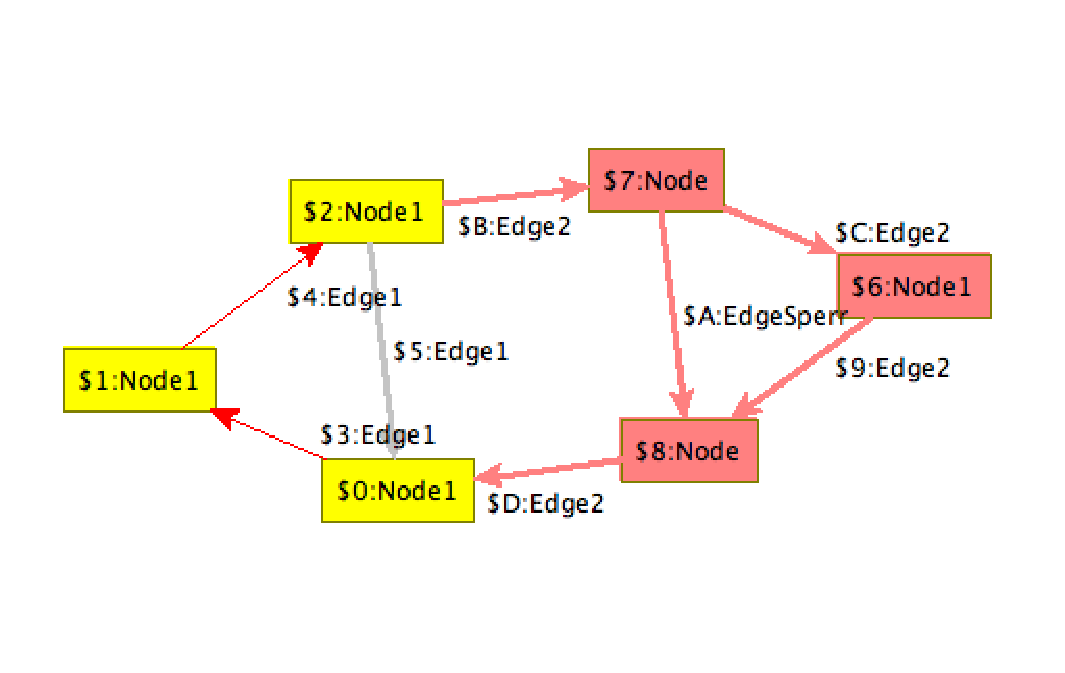
\includegraphics[width=\linewidth]{fig/debug2tra}}\parbox{0.375\linewidth}{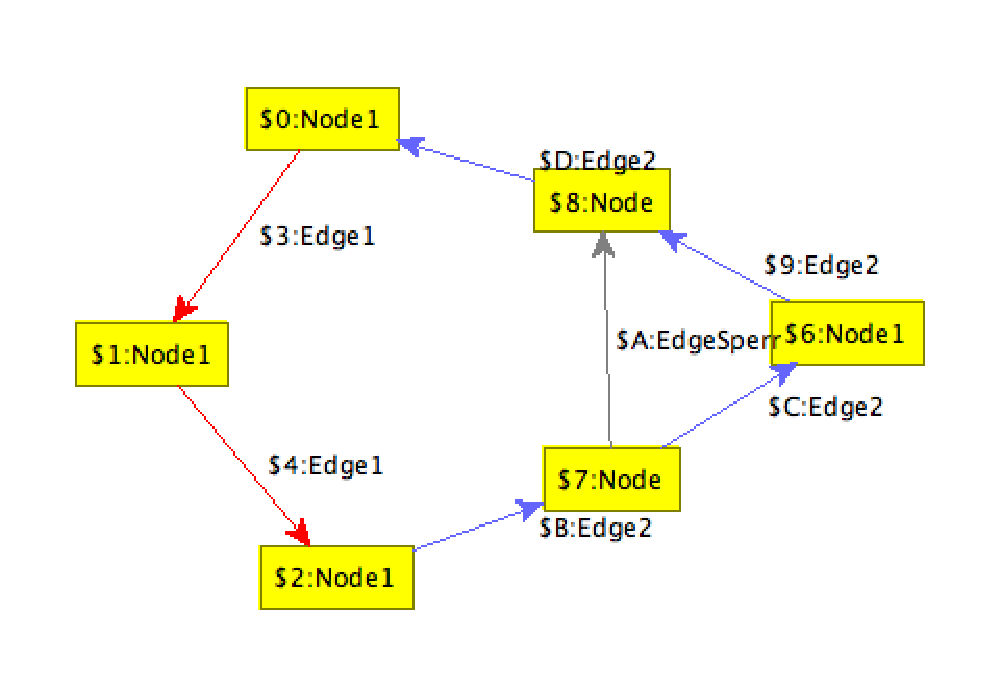
\includegraphics[width=\linewidth]{fig/debug3tra}}
\end{center}
The following table shows the ``break points'' of further debug commands, entered one after another:
\begin{center}
  \begin{tabular}{|l|l|} \hline
    \textbf{Command} & \textbf{Active rule} \\ \hline
    \texttt{s} & \texttt{makeFlake1} \\
    \texttt{o} & \texttt{beautify} \\
    \texttt{s} & \texttt{doNothing} \\
    \texttt{s} & \texttt{beautify} \\
    \texttt{u} & \texttt{beautify} \\
    \texttt{o} & \texttt{makeFlake2} \\
    \texttt{r} & --- \\ \hline
  \end{tabular}
\end{center}
\end{example}
\end{figure}

%\subsection{yComp}
%url; yFiles; java app, socket communication with shell debugger
%Find; goto node/edge; b�bbels;
%relayout; zoom: mousewheel; pane by holding middle mouse
%supported formats; vcg format
%ref to visualization commands, again: hierarchy
%copy some of the stuff from ycomp help?


